\documentclass[usenatbib,fleqn]{mn2e}
\usepackage{amsmath,amssymb}
\usepackage{graphicx}
\usepackage{epstopdf}
\epstopdfsetup{outdir=./figures/}
\graphicspath{{./figures/}}
\usepackage{url}
\usepackage{aas_macros}
\usepackage{astro}
%\usepackage{natbib}


\newcommand{\Mdot}{\dot{M}}
\newcommand{\eddr}{\dot{M}/\dot{M}_{\rm Edd}}
\newcommand{\Mdote}{\dot{M}_{\rm Edd}}
\newcommand{\Mdotb}{\dot{M}_{\rm bondi}}

\newcommand\lsim{\mathrel{\rlap{\lower4pt\hbox{\hskip1pt$\sim$}}
        \raise1pt\hbox{$<$}}}
\newcommand\gsim{\mathrel{\rlap{\lower4pt\hbox{\hskip1pt$\sim$}}
        \raise1pt\hbox{$>$}}}
\newcommand{\rs}{r_s}
\newcommand{\rb}{r_b}
\newcommand{\vw}{v_w}

\newcommand{\dxdy}[2]{\frac{\partial #1}{\partial #2} }
\newcommand{\ddr}[1]{\dxdy{#1}{r}}
\newcommand{\drhodt}{\dxdy{\rho}{t}}
\newcommand{\dpdr}{\dxdy{p}{r}}
\newcommand{\dvdr}{\dxdy{v}{r}}
\newcommand{\dsdr}{\dxdy{s}{r}}
\newcommand{\dphidr}{\dxdy{\Phi}{r}}

\newcommand{\ke}{\frac{v^2}{2}}
\newcommand{\kew}{\frac{v_w^2}{2}}

\newcommand{\gammaf}{\frac{\gamma}{\gamma-1}}
\newcommand{\gammafi}{\frac{\gamma-1}{\gamma}}
\newcommand{\cs}{\frac{p}{\rho}}
\newcommand{\Q}{q (\ke+\kew-\gammaf \cs)}

\newcommand{\kb}{k_{\rm b}}
\renewcommand{\mp}{m_{\rm p}}
\newcommand{\pc}{\rm pc}

\newcommand{\Menc}{M_{\rm enc}}
\newcommand{\rhostar}{\rho_*}
\newcommand{\Mstar}{M_{\star}}
\newcommand{\Mseight}{M_{\star,8}}
\newcommand{\Mbh}[1][]{M_{\bullet#1}}
\newcommand{\Mbheight}{M_{\bullet,8}}
\newcommand{\MbhNorm}{\frac{\Mbh}{10^8 \Msun}}

\newcommand{\phirs}{\frac{G \Menc}{\rs}}
\newcommand{\soi}{\rm soi}
\newcommand{\rsoi}{r_{\soi}}
\newcommand{\ff}{\rm ff}
\newcommand{\tff}{t_{\ff}}
\newcommand{\rIa}{r_{\rm Ia}}
\newcommand{\sigsoi}{\sigma_{\soi}}

\newcommand{\vwO}{v_{w,0}}
\newcommand{\kewO}{\frac{\vwO^2}{2}}
\newcommand{\x}{\frac{r_s}{\rsoi}}
\newcommand{\vwNorm}{\frac{\vwO}{\sigsoi}}
\newcommand{\vwOFH}{v_{w,0,500}}
\newcommand{\vwOFHexp}{\frac{\vwO}{500 \, {\rm km/s}}}

\newcommand{\pyear}{{\rm yr}^{-1}}
\newcommand{\tage}{t_{\rm age}}
\renewcommand{\th}{t_h}

\topmargin -1 cm
\defcitealias{WangMerritt:2004a}{WM04}	

\author[Generozov, Metzger, \& Stone]{Aleksey Generozov$\thanks{E-mail: ag@astro.columbia.edu}$, Brian~D.~Metzger, Nicholas Stone\\
Columbia Astropysics Labratory, Columbia University, 550 West 120th Street, New York, NY 10027}


\begin{document}
\title{Constraining Quiescent Supermassive Black Hole Environments.}
 \maketitle

\begin{abstract}
Abstract here 
\end{abstract}

 \begin{keywords}
 black hole physics --  galaxies: active
 \end{keywords}


\section{Introduction}
\label{sec:introduction}

%%Maybe active galaxies constitute 10% need reference here?
Supermassive black holes (SMBHs) are present in the centers of most,
if not all nearby galaxies (see reviews by,
e.g. \citealt{KormendyRichstone:1995a};
\citealt{FerrareseFord:2005a}). Roughly $\sim 1\%$ of these manifest
themselves as luminous Active Galactic Nuclei. However, quiescent
black holes constitute a silent majority.

In order to understand why most galaxies appear to be inactive, it is
necessary to understand the gas environment of black holes, as the gas
density around the black hole sets its accretion rate.  The accretion
rate also has implications for rate of black hole growth.
%AG:Perhaps need more detail here.

Constraints on the SMBH accretion rates at the low end of the SMBH
mass function also have implications for the black occupation
fraction.  For example, \citealt{MillerGallo+:2014a} used an observed
relation between $\Mbh$ and nuclear x-ray luminosity $L_x$ to
constrain the BH occupation fraction.  However, they extrapolate
(assuming a single power law) their observed relationship below their
detection threshold.  However, it is possible that the $L_x$-$\Mbh$
relationship steepens at smaller $\Mbh$, and thus the black hole
occupation fraction could be underestimated at low $\Mbh$.
%AG: In our model we obtain a steeper relationship, but we have difficulty matching the observed relationship above the detection threshold

The gas environment also plays an important role in determining
observables (light-curves, SEDs) from jetted tidal disruption events
(TDEs). These are bright flares that occur when a star passes within
the tidal disruption radius of the SMBH. A small fraction of events
are accompanied by the launch of a relativistic jet into the
circumnuclear medium (CNM) of the host galaxy.  As the jet propagates
into the CNM, a reverse shock propagates towards the back of the jet,
decelerating it. The CNM density profile will determine the final
Lorentz factor of the jet. This in turn will strongly affect the
duration of the observed synchotron radiation.

The gas in the vicinity of a black hole may come from several
sources. \citealt{Ho:2009a} proposes three different mechanisms (1)
Mass loss in winds (particularly from evolved stars) (2)
Stellar-stellar collisions in dense environments (3) Tidal disruptions
of stars. To estimate (a lower limit on the accretion rate),
\citealt{Ho:2009a} calculates the Bondi accretion rate based on
typical observed gas densities and temperatures taken from Chandra
X-ray observations. A second estimate is obtained from the wind mass
loss rate from the observed stellar densities. Both of the estimates
suggest that there is an ample reservoir of gas to power active
galactic nuclei in quiescent galaxies. This suggests that the lack of
the AGN activity is due to the fact that the accretion proceeds in a
radiatively inefficient mode.

Previous studies used Chandra observations to show that the Bondi
accretion power well-correlated with jet power
\citep{AllenDunn+:2006a,FujitaKawakatu+:2014a}. In these studies
temperature, and density information are inferred from Chandra x-ray
observations, while the jet power is inferred from the energy required
to inflate observed bubbles within the x-ray emitting gas.

However, this approach has limitations. Due to resolution issues it is
almost never possible to observationally determine the gas density at
the black sphere of influence, and such studies are forced to
extrapolate observed gas temperatures and densities to smaller scales.
In fact, the temperature profile is assumed to be flat inside of the
Bondi radius.  In reality, the cusp in the velocity dispersion near
the SMBH, should cause a cusp in the gas temperature profile (assuming
the kinetic energy of stellar winds is efficiently themalized in
shocks).
%%AG-give sense of scale.

Another approach to constraining the gas density around an SMBH is to
go from a stellar mass loss rate (motivated by observed stellar
densities) to a steady-state gas profile. This approach was taken by
\citealt{Quataert:2004a,De-ColleGuillochon+:2012a,ShcherbakovWong+:2014a}.

% In this study we perform hydrodynamic modeling to solve for the
% steady-state gas density, temperature and velocity profiles near the
% SMBH sphere of influence, for a sample of nearby, quiescent
% galaxies. We a adopt the model used by \cite{Quataert:2004a} for the
% galactic center: gas is supplied by stellar winds, which collide,
% shock heat, and thermalize.
We take the same approach. To the best of our knowledge a systematic
study of the parameter space of central galaxy properties. Thus, we
compute central density profiles for a broad sample of galaxies from
\citealt{WangMerritt:2004a}--henceforward
\citetalias{WangMerritt:2004a}.  This allows us to relate the central
stellar properties (e.g. the slope of the stellar density) to the
central gas properties.

For each galaxy in our chosen sample, we find a steady state gas
profile. Typically an inflow-outflow structure is established. The
stellar ejecta inside of the stagnation radius ($\rs$) will be
accreted, while that outside $\rs$ will be driven out with the
outflow.  It is often assumed that the gas properties at the Bondi
radius, $\rb$ set the accretion rate. However, physically it is really
$\rs$ which sets the accretion rate. Typically this lies within a
factor of a few of the $\rb$.  This means that with perfect knowledge
of the gas profile the $\Mdotb$ is typically a good approximation to
the actual accretion rate $\Mdot$.  However, using extrapolations of
the observed gas temperature and density to estimate $\Mdot$ may cause
systematic order of magnitude errors in the inferred accretion rate.

The location of $\rs$ and hence the accretion rate is quite sensitive
to the assumed heating rate.  Physically, the heating rate of the gas
would vary from galaxy to galaxy. For example, SNe Ia may be a large
source of energy for the gas. However, this will be only be the case
for larger black holes for which the gas inflow time is smaller than
the time between successive Ias. Thus, for smaller black holes, the
effective gas heating rate may be considerably smaller. We
investigate the effect of changing rate of energy injection on the gas
density profiles.

We compare our calculated gas profiles to those inferred from Chandra
X-ray observations by \citealt{AllenDunn+:2006a} and
\citealt{RussellMcNamara+:2013a}. Additionally, we chack how well our
results are able to reproduced relationships between $L_x$ and $\Mbh$
in \citealt{MillerGallo+:2014a}. In performing these comparisons we
hope to determine how well the gas environments of quiescent galaxies
may be understood using the relatively well understood physics of
stellar winds and supernova heating.
 %%AG--say something about x-ray observations. 


\section{Sample}
We start with a sample of 61 galaxies from
\citetalias{WangMerritt:2004a}, as subset of a larger sample of
galaxies from \citealt{FaberTremaine+:1997a}. These are nearby
elliptical galaxies, observed with the Hubble WFPC2.

We focus on elliptical galaxies to isolate the effect of mass loss
from a relatively old stellar population, avoiding additional gas
flowing in from star formation on larger scales.

For each galaxy in the sample we take the surface brightness
parameterization given in Table 1 of
\citetalias{WangMerritt:2004a}. The parameterization is a Nuker law

\begin{equation}
  I(\xi)=I_b 2^{(\beta-\Gamma)/\alpha} \xi^{-\Gamma} (1+\xi^\alpha)^{-(\beta-\Gamma)/\alpha}, \xi=\frac{r}{r_b}.
\end{equation}

This is a broken power law which transitions from an inner power law
slope, $\gamma$, to an outer power law slope, $\beta$, at a break
radius, $\rb$.  The corresponding (spherically symmetric) stellar
density, $\rhostar\sim r^{-1-\gamma}$ for $r \ll \rb$ and
$\rhostar\sim r^{-1-\beta}$ for $r \ll \rb$.  $\gamma\simeq1$ for cusp
galaxies, while $\gamma\simeq0$ for core galaxies.
%AG:Is there a systematic dependence of beta on galaxy type$.

From the surface brightness profile, we follow the same procedure as
\citetalias{WangMerritt:2004a} to compute the spatial stellar density
and stellar mass profile, both of which are used in our model.

%% AG--some discussion of alternate parameterizations.  My intuition
%% is that for our purposes the parameterization should not
%% matter. But some discussion of alternate possibilities could
%% prevent Alistar Graham from yelling at us.

\section{Model}
\label{sec:model}
We use the same model as \citealt{Quataert:2004a} to find a steady
state gas density near the SMBH for each of the galaxies within our
sample.  Gas is supplied by winds from the stellar population in the
galactic center. Assuming a rate of mass injection, $q$, spherical
symmetry and an ideal gas equation of state.

\begin{align}
&\drhodt+\frac{1}{r^2}\dxdy{\rho r^2 v}{r}=q\\
&\rho \frac{dv}{dt}=-\dpdr-\rho \dphidr-q v\\
&\rho T \frac{ds}{dt}=q\left[\ke+\kew+\gammaf \cs \right]
\end{align}

These or similar equations have been solve many times in the
literature (e.g. \citealt{HolzerAxford:1970a,Quataert:2004a,De-ColleGuillochon+:2012a,ShcherbakovWong+:2014a}). \citealt{ShcherbakovWong+:2014a}
adds additional terms to account for thermal conduction and radiative
cooling. However, we find that radiative cooling may be neglected for
a large portion of our parameter space--\S~\ref{sec:cooling}.
Additionally thermal conduction may be cut off by magnetic field
lines--\S~\ref{sec:conduction}

$q$ represent the rate of injection of gas mass per unit volume, and
is derived from the stellar density, $\rho_*$, using

\begin{align}
q=\frac{\eta \rho_*}{t_h}
\end{align}

%%AG $eta/th$ is the specific of rate of mass return to the ISM.  Ciotti et al. 1991 -- see in particular Table 2. 
Where $t_h$ is the Hubble time, and $\eta$ is an efficiency parameter--for a stellar population between 2-15 Gyr old, this number will lie in the range $\sim$0.1-1 (see Appendix~\ref{app:eta}). We adopt $\eta=1$. However, scaling $\eta$ by some factor, would simply scale the $\rho$ by the same factor and otherwise leave the solution unchanged. 

$\vw^2/2$ encapsulates heating in our simulation. We take $\vw^2=\sqrt{\sigma(r)^2+v_{w,0}^2}$ where $\sigma(r)$ corresponds to the velocity dispersion of the stars and $v_{w,0}$ accounts for additional heating sources (ms pulsars, SNe Ia, etc.)  We approximate $\sigma(r)$ to be given by $G \Menc/r=G(\Mbh+\Mstar)/r$, where $\Mbh$ is the mass of the SMBH and $\Mstar$ is the stellar mass inside radius $r$. 

% {\bf NCS: here is some added detail about the role of stellar mass
% functions in the model}

% if we consider different star formation scenarios (for example,
% continuous star formation) or different IMFs, it will change.  Once
% these free parameters are specified, however, we can answer an
% important question: do young stellar populations increase or
% decrease the SMBH feeding rate $\dot{M}$?  Clearly, $\eta(t)$ is
% larger for young stellar populations, but these stars also have high
% wind velocities that diminish the stagnation radius.  Crudely
% approximating $v_{\rm w}=200~{\rm km~s}$ for $m_{\rm max} <
% 10M_{\odot}$ and $v_{\rm w}=1000~{\rm km~s}$ for $m_{\rm max} >
% 10M_{\odot}$ (motivated by the transition from dust-driven wind loss
% on the AGB to line-driven wind loss on the main sequence), we can
% employ the relation $\dot{M} \propto \eta(t) r_{\rm
% s}^{2-\Gamma}\propto \eta(t) v_{\rm w}^{-4+2\Gamma}$ (where $\rho_*
% \propto r^{-\Gamma}$) to determine the impact of stellar ``youth''
% on SMBH feeding rates.
%
%\begin{figure}
%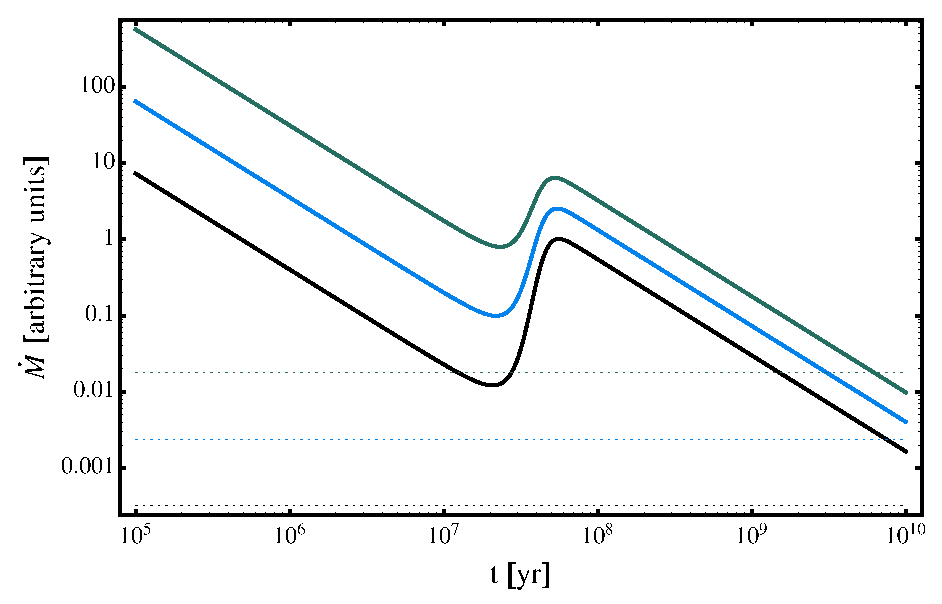
\includegraphics[width=\columnwidth]{NickPlot.eps}
%\caption{\label{NickPlot} SMBH feeding rates $\dot{M}=\eta(t) \times M_*(r_{\rm s})$, in arbitrary units.  The green, blue, and black curves are for galaxies with $\Gamma$ values of $0.1$, $0.5$, and $0.9$, respectively.  Solid curves represent impulsive-mode star formation, while dotted curves represent continuous-mode star formation.}
%\end{figure}
%
%%In Fig. \ref{NickPlot} we plot $\dot{M}$, in arbitrary units, as a function of time, for three different stellar density profiles $\Gamma = \{1.1, 1.5, 1.9\}$ (which are normalized to have the same mass at an influence radius $r_{\rm soi}=10~{\rm pc}$ around a $10^7M_\odot$ SMBH).  We parametrize the wind velocity as 
%\begin{equation}
%\frac{v_{\rm w}}{\rm km~s^{-1}}=600-400\tanh\left( \frac{t-10^{7.5}~{\rm yr}}{10^{7}~{\rm yr}}\right).
%\end{equation}
%The ``impulsive burst'' mode of star formation produces large ($\sim 10$) differences between the three $\dot{M}$ curves at early times, when $r_{\rm s}$ is small, but smaller ($\sim 3$) differences at late times, when $r_{\rm s}$ is large.  We also plot, as dotted curves, a simple model for the ``continuous'' mode of star formation, where mass loss is calculated as $\bar{\eta} = \int\eta(t)dt/t_{\rm h} \approx 4$ and an average energy injection in the wind is calculated as $\bar{v_{\rm w}^2}=\int\eta(t)v_{\rm w}^2(t)dt/\bar{\eta} \approx (800~{\rm km~s}^{-1})^2$.  Interestingly, the continuous mode of star formation produces small differences from late-time $\dot{M}$ seen in cusp galaxies with impulsive star formation; however, continuous mode star formation decreases late-time $\dot{M}$ by an order of magnitude relative to impulsive star formation in core galaxies.

\section{Solutions}
\subsection{Analytics: Flow properties at $\rs$}
It is possible to derive an analytic expression for the steady-state stagnation radius, $\rs$, in terms of $v_w$ and the power law slope of the density (at $\rs$) $n$.   We summarize the main results here and place the detailed derivation in Appendix~\ref{app:rs}.

The temperature at the $\rs$ is given by

\begin{align}
 &\frac{\kb T}{\mu \mp}=\gammafi \kew \label{eq:tstag}\\
 &T=6 \times 10^6 {\rm K} \, \mu \, \left({\frac{\vw}{500 \,{\rm km/s}}}\right)^2 
\end{align}

We may also write an (implicit) analytic expression for $\rs$
itself. Let  $\eta=v_{w,0}/\sigma_{\rm soi}$. Then 

\begin{align}
\x=\frac{1}{\eta^2 n}\left[ (1+\Mstar(\rs)/\Mbh)\left(A-\frac{n}{2}\right)-B\right]
\label{eq:stag_analytic}
\end{align}

Where A and B are are constants, which depend on the nuker $\gamma$
and the adiabatic index of the gas (see Appendix~\ref{app:rs})  $\Mstar << \Mbh$ at the stagnation radius, the relationship between $\rs$ and $\vw$ is greatly simplified. 

\begin{align}
&\rs=\frac{7}{2}\frac{G \Mbh}{n \vw^2}\\
&\simeq 6 \, \pc \left(\MbhNorm\right) \left(\vwOFH\right)^{-2}
\label{eq:stag_simple}
\end{align}

This relationship will hold as long as $\vw > \sigma(\rsoi)$, or equivalently (from the $M-\sigma$ relationship) $\vwO > \left(\frac{\Mbh}{10^8 \Msun}\right)^{1/5} 200 {\rm \,  km/s}$.

$\Mdot$ flowing towards the hole is given by

\begin{align}
\dot{M}=\frac{\eta \Menc(\rs)}{\rs}
\end{align}

In physical units this may be approximated as 

\begin{align}
\dot{M}\simeq
\begin{cases}
   1.5 \times 10^{-3}  \left(\Mbheight\right)^{1.9}
   \left(\vwOFH\right)^{-4} \eta \Msun \, \pyear& \text{for core galaxies} \\
   3.3 \times 10^{-3} \left(\Mbheight\right)^{1.4}
   \left(\vwOFH\right)^{-2} \eta \Msun \, \pyear  & \text{for cusp
     galaxies} 
 \end{cases}
\label{eq:mdot_analytic}
\end{align}

In our model the accretion onto the black hole may be approximated as
the gas mass enclosed inside $\rs$ divided by the free-fall time at $\rs$.

\begin{align}
&\dot{M}\simeq\frac{(4 \pi/3) \rs^3 \rho(\rs)}{t_{\ff}(\rs)}
\label{eq:mdot_gas}
\end{align}

Finally, using Equations~\ref{eq:tstag} and \ref{eq:mdot_analytic}, we
may obtain a scaling relationship for $\rho(\rs)$. 

\begin{align}
\rho(\rs)\simeq
\begin{cases}
2.5 \times 10^{-24} \Mbheight^{-0.14} \vwOFH^{-1} \eta \, {\rm g \, cm^{-3}}& \text{for   galaxies}\\
5.5 \times 10^{-24}  \Mbheight^{-0.56} \vwOFH    \eta \, {\rm g \,cm^{-3}} & \text{for cursp galaxies}
\end{cases}
\label{eq:rhors}
\end{align}


\subsection{Comparison with Bondi Accretion}
The Bondi accretion rate, $\Mdotb$ in terms of the Bondi radius $\rb=G
M/c_s^2$ is 

\begin{align}
\Mdotb=4\pi \lambda r_b^2 \rho(r_b) v_{\rm ff}(r_b).
\end{align}

We may rewrite Equation~\ref{eq:mdot_gas} as follows

\begin{align}
&\dot{M}\simeq\frac{(4 \pi/3) \rs^3 \rho(\rs)}{t_{\ff}}\\
&=\frac{4 \pi}{3} \rs^2 \rho(\rs) v_{\ff}(\rs)
\end{align}

Note that to within factors of order unity this is the same as Bondi formula, except $\rb$ is replaced by $\rs$. 
From Equation~\ref{eq:stag_simple}

\begin{align}
\rs=\frac{7}{2}\frac{G \Mbh}{\vwO^2}.
\label{eq:rs_simple}
\end{align}

Where have set the power law slope of the gas density, $n$, to 1.  At $\rs$ we have

\begin{align}
\kew=\frac{c_s^2}{\gamma-1}
\end{align}

Thus, $\cs(\rs)\simeq \vw(\rs)$. This means that $\dot{M}$ in our model is quite close to $\Mdotb$


%% AG-Apparently even in the low heating case, it is still possible to
%% an outflow (from the analytic results above the gas density must be
%% quite steep in this case). However, at low heating we will probably
%% become subject to a cooling instablity.  AG-I believe that in the
%% case of core galaxy, the negative root of the quadratic should be
%% taken...

\subsection{Numerics: Full numerical solution for galaxy sample}
We compute solution for our sample of galaxies for three different values of $v_{w,0}$: 1000 km/s, 500 km/s, and 200 km/s. 

We show show three representative profiles in Figure~\ref{fig:profiles} below. 

We show the numerical results for $\x$ vs. $\eta$ in the top panel of
Figure~\ref{fig:stag}.  The three different colors represent the three
different chosen values of $\vwO$. The square points represent cusp
galaxies, whereas the triangles represent core galaxies.  The solid
line is a power law fit through the cusp galaxies, while the dotted
line is a power law fit through the core galaxies.

Using the slope of the density profile, at the stagnation radius we
may use Equation~\ref{eq:stag_analytic} to compute $\x$
analytically. We plot the fractional difference between the numerical
and analytic results for $\x$ for each galaxy in the bottom panel of
Figure~\ref{fig:stag}.  Generally, the agreement is quite good
(especially for $\vwO$=1000 km/s and $\vwO$=500 km/s), providing a
useful check of the numerical results.

%%AG: Describe conservation checks to additionally validate the results.



\begin{figure}
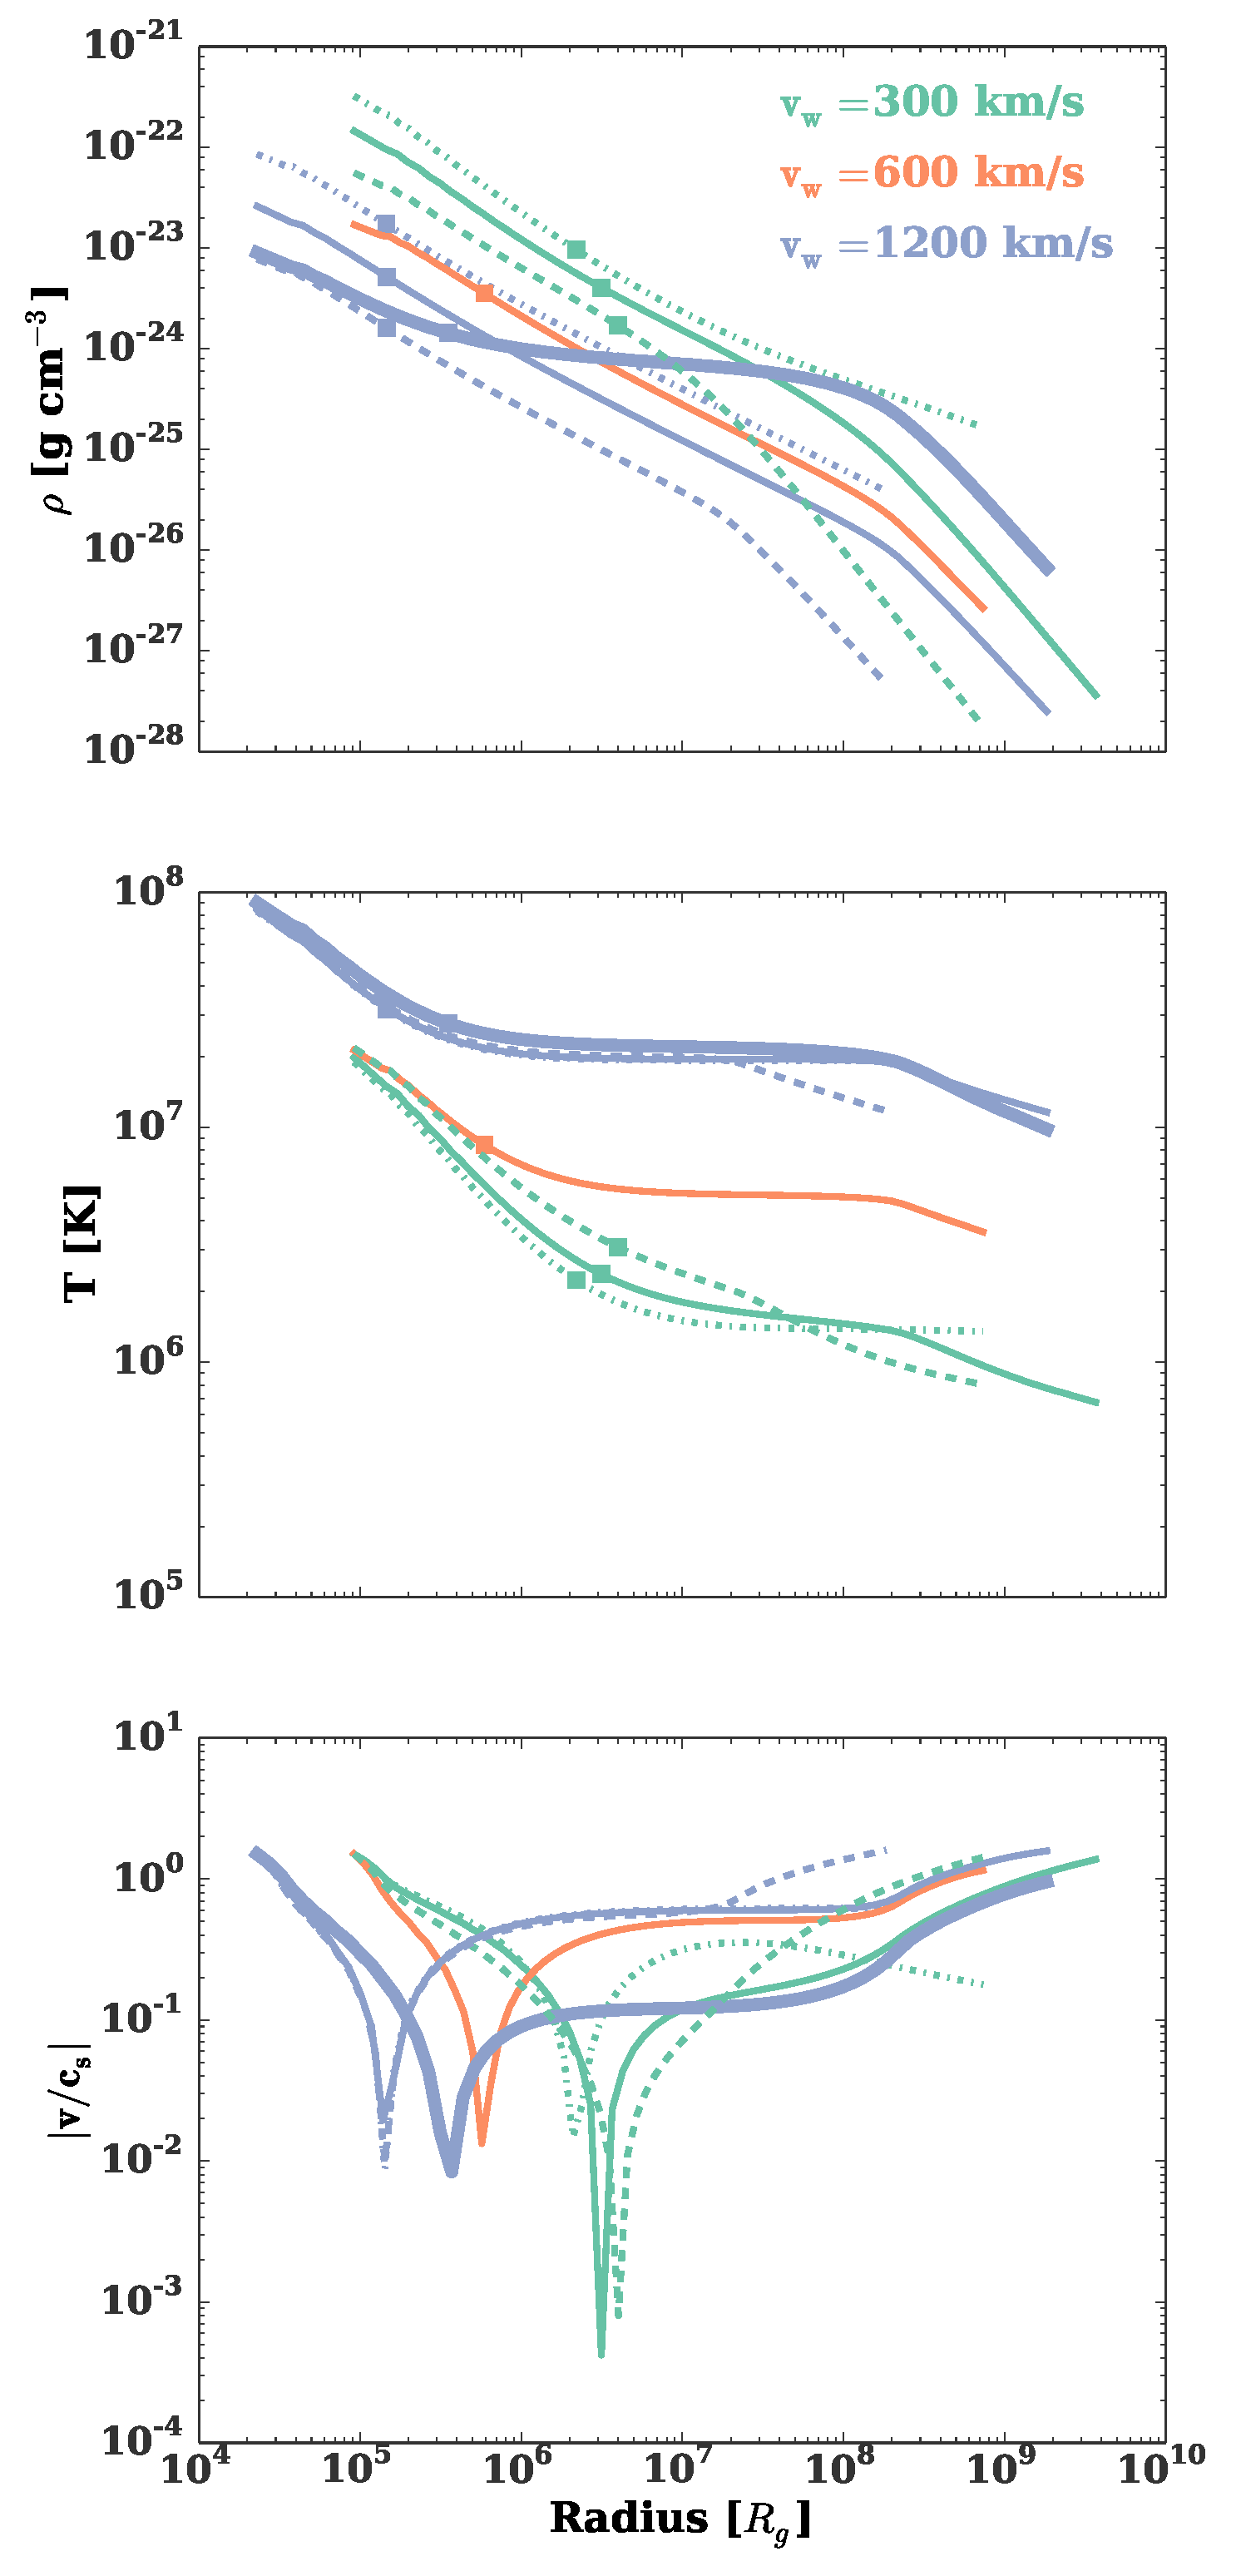
\includegraphics[width=\columnwidth]{profiles.eps}
\caption{\label{fig:profiles}Radial for three different galaxies:
  NGC1172, NGC4478, and NGC3115. Solid curves correspond to $v_w$=1000
  km/s.  The Dot-dashed curve corresponds to $v_w$=200 km/s. Top
  panel: Density; Middle Panel: Temperature; Bottom Panel: X-ray
  luminosity enclosed within radius $r$.}
\end{figure}

\begin{figure}
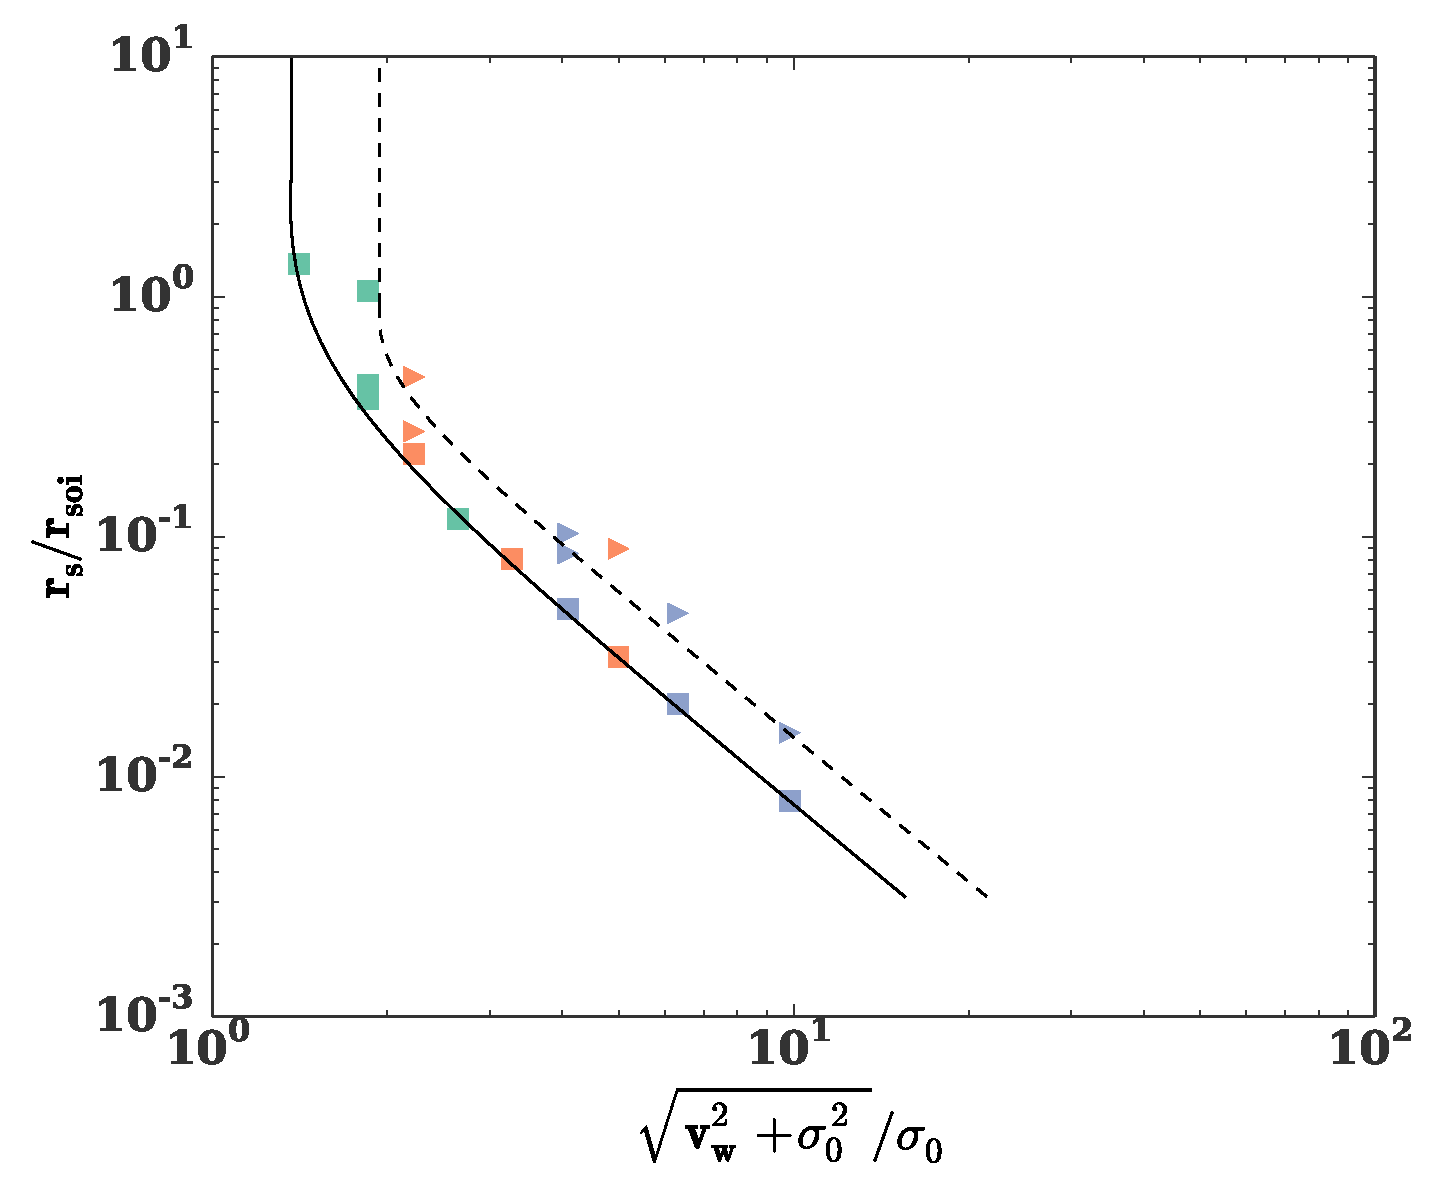
\includegraphics[width=\columnwidth]{rs.eps}
\caption{\label{fig:stag}$\x$ vs. $\vwNorm$}
\end{figure}


\section{Discussion}
\subsection{Heating}
We now discuss potential sources of heating and discuss how different
physical sources of heating would lead to different values of
$\vwO$. For each heating source from the heating rate per unit volume
$e$ we may estimate the corresponding $\vwO$, using

\begin{align}
&\frac{q \vwO^2}{2}=e\\
&\frac{\eta \rhostar \vwO^2}{2 t_h}=e
\label{eq:vw_eff}
\end{align}

We estimate the value of the $\vwO$ for different physical heating
sources below.

\begin{enumerate}
\item \emph{Stellar winds} The contribution to the heating rate from
  the red giant winds themselves will be negligible, as red giants
  have wind velocities $\lsim 40$ km/s.

  Although red giant winds dominate the mass budget, winds from main
  sequence stars may make a significant contribution to the energy
  budget, with wind velocities $\sim 100-150$ km/s
  \citep{NaimanSoares-Furtado+:2013a}.

\item \emph{MS Pulsars} The spin down power of millisecond pulsars
  (MSPs) could potentially be an important heating source. Assuming a
  spin-down luminosity $L_{\rm sd}$ and $n_{\rm msp}$ MSPs per unit
  mass

\begin{align}
e=L_{\rm sd} n_{\rm msp} \rhostar.
\end{align}

Then we may obtain the $\vwO$ from Equation~\ref{eq:vw_eff}. m

\begin{align}
\vwO=\sqrt{\frac{2 t_h n_{\rm msp} L_{\rm sd}}{\eta}}
\end{align}

There may be as many 30,000 MSPs in the Milky way, which would give
$n_{\rm msp}\simeq3 \times 10^{-41} $ MSPs g$^{-1}$. Even if we
optimistically take $L_{\rm sd}\simeq 10^{35}$ ergs/s, and $\eta$=0.1,
we would get $\vwO\simeq40$ km/s, which means heating by MSPs is
negligible.

Also, MSPs may also be dissociated in the galactic center...
%%Also low thermalization efficiency inferred in 47 Tuc by Naiman et al.

\item \emph{Type Ia SNe} From he energy injected per Ia SNe,
  $E_{\rm Ia}$, and the SNe rate, $R_{\rm Ia}$

\begin{align}
e=R_{\rm Ia} E_{\rm Ia} \rhostar
\end{align}

Then from Equation~\ref{eq:vw_eff}

\begin{align}
\vwO=\sqrt{\frac{2 t_h R_{\rm Ia} E_{\rm Ia}}{\eta}} \label{eq:vw_sne}
\end{align}

Following \citealt{ShcherbakovWong+:2014a}, $E_{\rm Ia}=10^{51}$ ergs
and $R_{\rm Ia}\simeq 4 \times 10^{-14} \Msun^{-1}$ yr$^{-1}$, which
gives $\vwO\simeq 230 \, \eta^{-1/2}$ km/s (For $\eta=0.1$ this
corresponds to $\vwO\simeq$ 500 km/s.
 %Perhaps it would be best to adopt a fiducial eta=0.1--this may be more straightforward from the pov of both heating and cooling.

 As noted in \citealt{ShcherbakovWong+:2014a}, SNe energy injection
 cannot necessarily be treated as constant throughout time and space,
 since the flow time-scale may be short compared to the time between
 successive SNe Ia.

There will be some radius, $\rIa$, where the dynamical timescale of
the flow becomes comparable to the time between successive Type Ia
SNe.  If the stagnation radius ($\rs$) of the flow is outside of
$\rIa$ then SNes will provide a steady contribution to $\vwO$

The timescale between successive Type Ia SNes  is

\begin{align}
t_{\rm Ia} \sim 2.5 \times 10^5 \Mseight^{-1} \; {\rm yrs}.
\end{align}

The dynamical time is given

\begin{align}
  t_{\rm dyn} \sim r/\sigma \sim G \Mstar/\sigma^3 \sim 5 \times 10^4
  \Mseight \sigma_{200}^{-3} \; {\rm yrs}.
\end{align}

Therefore,

\begin{align}
  r_{\rm Ia} \sim G \Mstar{}_{,\rm Ia}/\sigma^2 \sim 4
  \sigma_{200}^{-1/2} \; {\rm pc}
\end{align}

The stagnation radius scales linearly with $\Mbh$ (see
Equation~\ref{eq:stag_simple}), while the $\rIa$ is roughly
constant. For small $\Mbh$, $\rs$ is well inside $\rIa$ and SNes will
not contribute to the $\vwO$.  Above $\sim10^8 \Msun$ SNes will
represent an important contribution to the overall heating.
% Thus, for $\Mbh=10^6 \Msun$, we may have $\vwO\simeq 100$ km/s with
% heating mostly coming from main sequence winds. On the other hand,
% for $\Mbh \gsim 10^8 \Msun$, we may have $\vwO\simeq 500$ km/s, with
% the main contribution coming from type Ia SNe. These two regimes are
% illustrated in Figure~\ref{fig:vw_eff}.
%\end{enumerate}

\item \emph{Overall Heating Rate} The overall value of $\vwO$ has
  contributions from Type Ia SNes and main sequence winds.  The
  relative contributions will depend on both the age of the stellar
  population, $\tage$, and $\Mbh$.  This is illustrated in
  Figure~\ref{fig:vweff}. For black hole masses below $10^7 \Msun$ SNe
  Ia will not contribute to $\vwO$ as the flow time scale is short
  compared to $t_{\rm Ia}$, and the heating is dominated by main
  sequence winds (with $\vwO\simeq 100$ km/s).  On the other hand, for
  $\Mbh \gsim 10^8 \Msun$, heating from Ias becomes important, as
  $\rs>\rIa$.  In this regime, we add the $\vwO$ values from SNe Ias
  and from main sequence winds in quadrature. $\vwO$ from SNe Ia's
  depends on the rate of mass loss ($\eta$), which is in turn a
  function of $t_{\rm age}$. This dependence is why the effective
  $\vwO$ increases with $\tage$ for large $\Mbh$.

For very young stellar populations ($\tage \lsim 10^7$ years),
$\vwO\simeq 1000$ km/s due to contributions from line driven winds
from high mass main sequence stars.

\begin{figure}
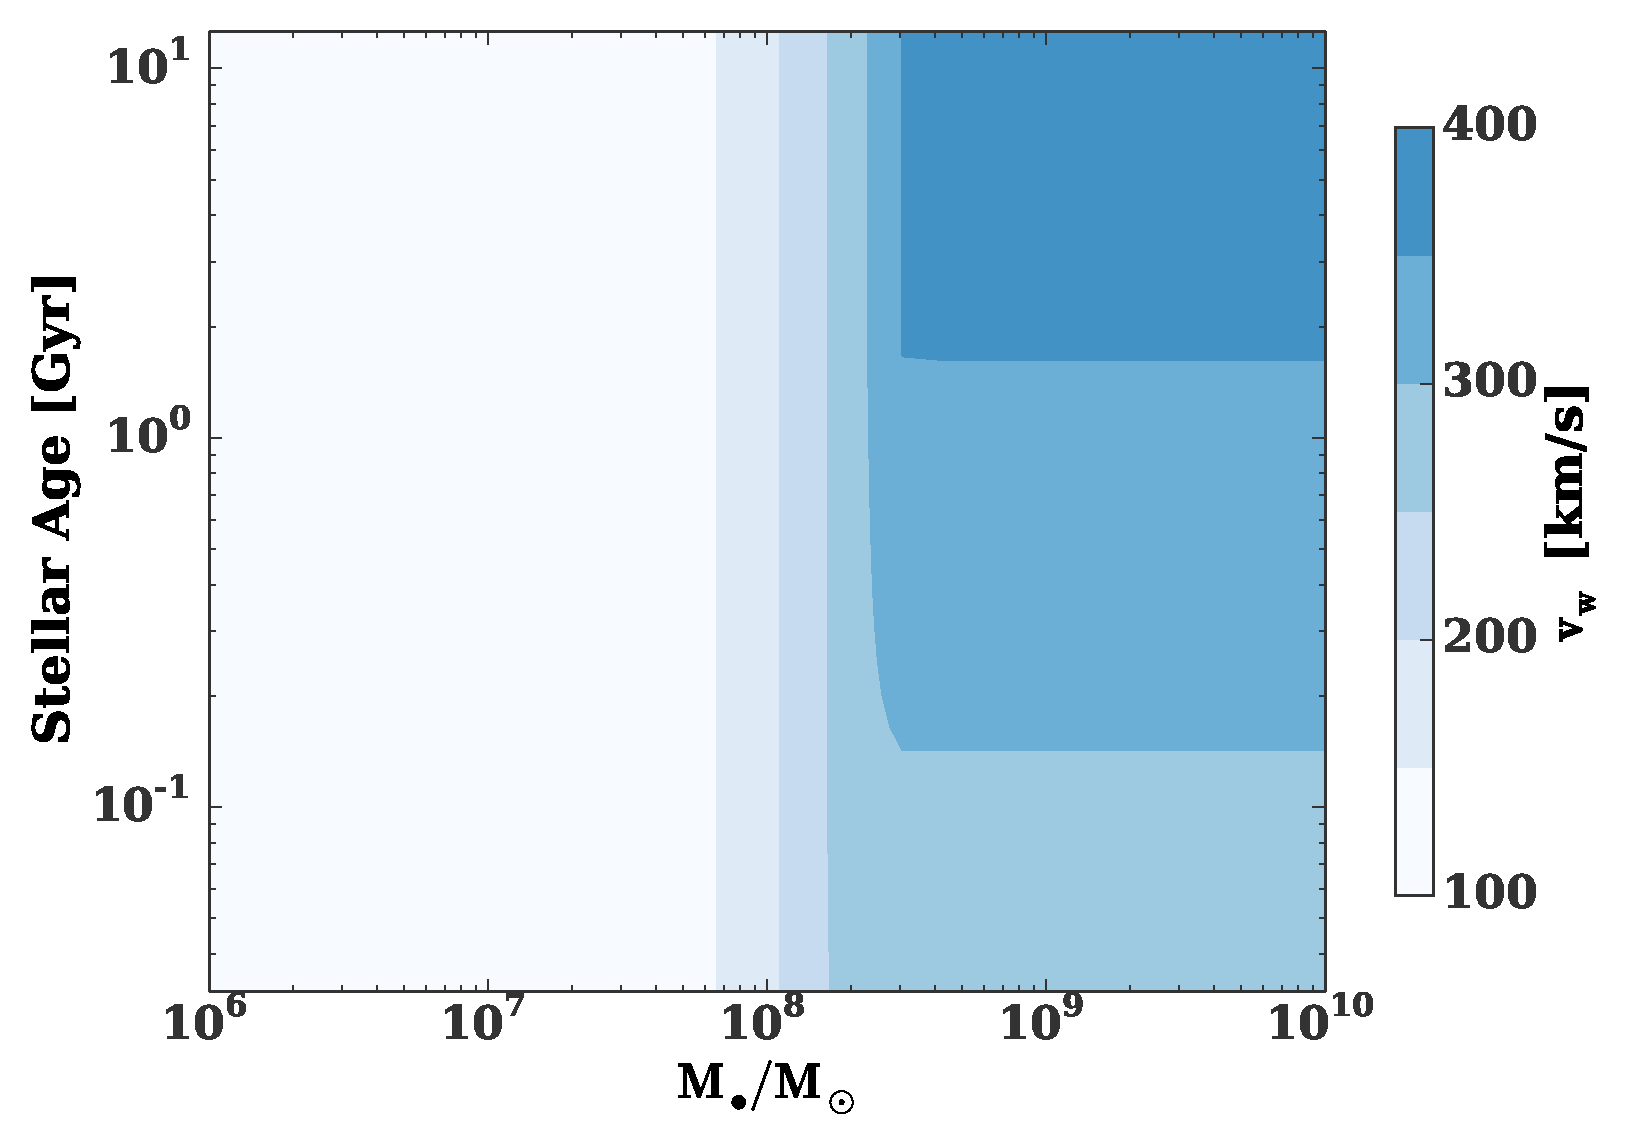
\includegraphics[width=\columnwidth]{vw-contour.eps}
\caption{\label{fig:vweff} Overall $\vwO$ for $\Mbh$-Stellar Age parameter space.}
\end{figure}

% AG-I am not comfortable saying type Ia SNe's don't contribute to
% heating for smaller mass BHs. If the cooling time for the SNe is
% long then it would be wrong to ignore the SNe contribution. The
% difference would be that the SNe heating would just be less steady.
% AG-Thornton and http://arxiv.org/pdf/1402.6695v2.pdf...
\end{enumerate}

\subsection{Mass accretion rate}
For each of our solutions, we may calculate the accretion rate
$\dot{M}$ onto the SMBH. We show $\Mdote$ vs. $\Mbh$ as a function of
black hole mass for our three chosen values of the $\vwO$ (200 km/s,
500 km/s, and 1000 km/s). The results are shown in
Figure~\ref{fig:mdot_mass}.  Note that $\dot{M}\sim\vwO^{-2}$ for a
cusp galaxy and $\dot{M}\sim\vwO^{-4}$ for a core galaxy. Thus, the
mass accretion rate will be a sensitive function of the assumed
heating rate.
%%AG-The variation in accretion rate for w/ vw for core galaxies is comparable to that of cusp galaxies and belies the steep dependence stated above.
%%AG-Note separation of cores and cusps (at vw=1000 km/s, where there are enough core galaxies for this comparison to be made). Also, note that the spread in core galaxies is far larger.

The accretion rate is proportional to the stellar mass enclosed inside
of $\rs$, so for core galaxies $\dot{M}\sim \Mbh (\rs/\rsoi)^{2}$,
while for cusp galaxies $\dot{M}\sim \Mbh (\rs/\rsoi)$.  This steeper
dependence is enough to offset the tendency for core galaxies to have
a larger $\rs/\rsoi$ for fixed $\eta$ (see
Figure~\ref{fig:stag}). Therefore, for $\rs/\rsoi<1$ core galaxies
would have a smaller $\dot{M}$ than cusp galaxies.  For $\vwO=1000$
km/s, core galaxies have a smaller accretion rate for a given black
hole mass.

We find there is a trend of $\eddr$ increasing towards higher black
hole masses. However, previous work suggests a downsizing trend: for
quiescent galaxies $L_X \sim \Mbh^\alpha$, where $\alpha\simeq
0.7-0.8$ \citep{MillerGallo+:2014a}. If $L_X\sim\dot{M}^2$, this would
suggest $\eddr\sim \Mbh^{-0.6}$. In contrast for fixed $\vwO$ and
$\eta$ we obtain that $\eddr\sim \Mbh^{0.5-1}$. One possible solution
is that $\eta$ decreases with $\Mbh$. $\dot{M}$ scales linearly with
$\eta$, so we would need to have $\eta\sim \Mbh^{-1}$ to explain the
observed downsizing trend.

\begin{figure}
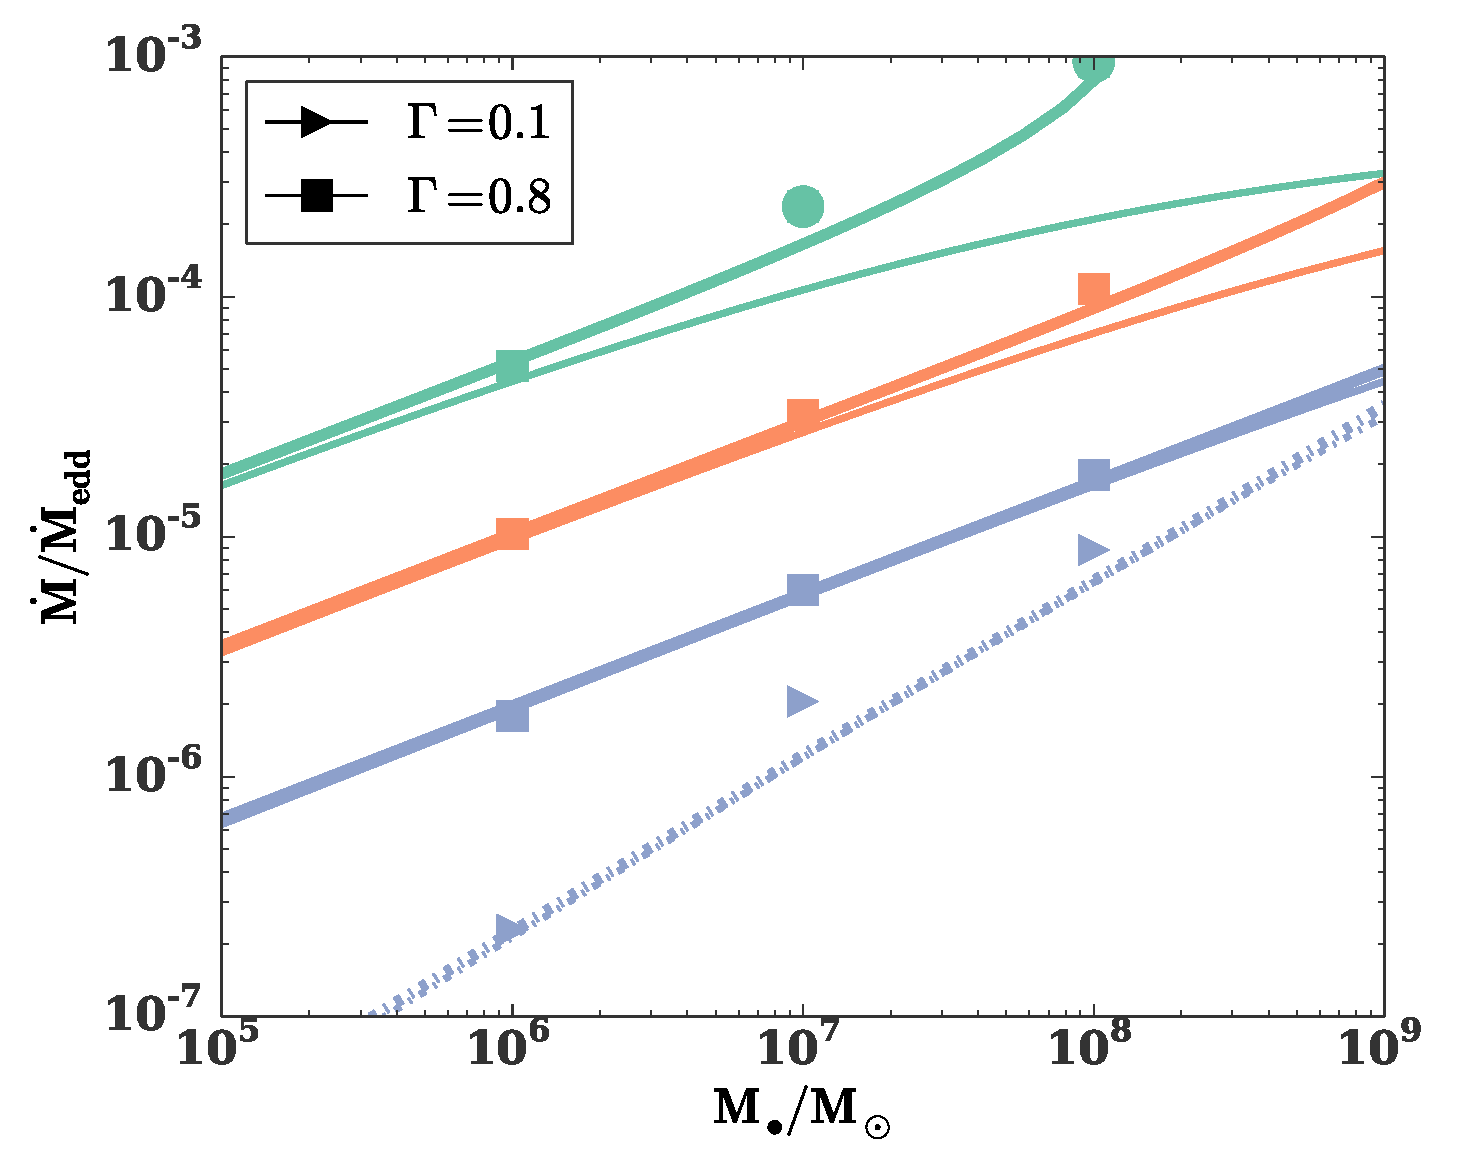
\includegraphics[width=\columnwidth]{mdot_mass.eps}
\caption{\label{fig:mdot_mass}$\eddr$ vs. $\Mbh$}
\end{figure}

%%AG:  Also want to include a plot of x-ray luminosity (less abstract than the accretion rate). 

\subsection{Comparison with observations}
\citealt{AllenDunn+:2006a} use Chandra x-ray observations to infer the
temperature and density profiles for nine nearby x-ray luminous
elliptical galaxies.  Five of the galaxies in their sample overlap
with that in \citetalias{WangMerritt:2004a}.

We may compare our results for the $T$ and $\rho$ profiles with those
inferred from observations for the overlapping galaxies.  Note that we
we have two free parameters ($\eta$ and $\vwO$ in our model and thus
we can can always match $T$ and $\rho$ at least one point.  We
generally find that $\vwO=500$ km/s (as would be expected from SNe Ia)
gives rough agreement with the observed temperatures.  Thus, we choose
$\vwO=500$ km/s.  We choose an $\eta$ so that our solution would be
consistent with the observed density profiles. The comparison is shown
in Figure~\ref{fig:allen_compare}.
%%AG-The chosen properties, in particular eta may be summarized in a table.


\begin{itemize}
\item \emph{NGC4486} %eta=0.2
  On scales of $\sim1$ kpc the density profile in
  \citealt{AllenDunn+:2006a} is shallower than in our model. Our model
  has a break in the gas density at $\sim 300$ pc--near the location
  of the Nuker break radius for this galaxy at 560 pc. There is an
  observed break in the density, but on a scale of a few kpc.

  In contrast to a naive extrapolation of the observed $T$ and $\rho$
  to smaller scales, our models have $T$ and $\rho$ monotonically
  increasing towards the galactic center. The increase in $T$ is due
  to the increased velocity dispersion (and thus increased heating)
  towards the galactic center.
\end{itemize}

\begin{figure*}
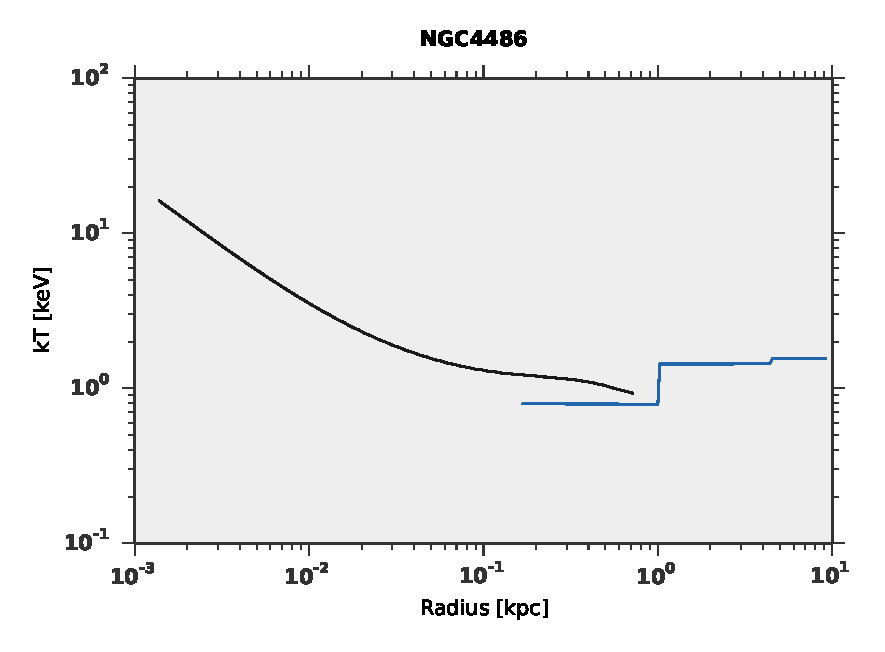
\includegraphics[width=\columnwidth]{T_compare.eps}
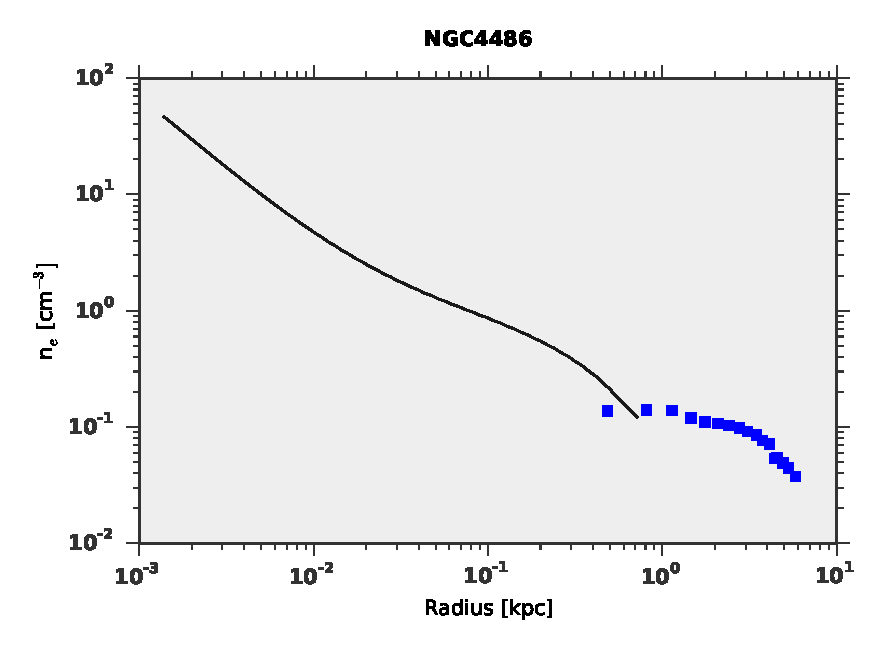
\includegraphics[width=\columnwidth]{dens_compare.eps}
\caption{\label{fig:allen_compare} Comparison of $n_e$ and $T$ to the \citealt{AllenDunn+:2006a}}. 
%%AG in the future we will have to be carfeful of the mean molecular weight.
\end{figure*}


 
\subsection{Cooling}
\label{sec:cooling}
In our models stellar winds collide, shock heat, and thermalize. The
rate of energy injection (parameterized by $\vwO$) sets a
characteristic temperature--see Equation~\ref{eq:tstag}.  For a given
amount of injected mass, the energy input from shock heating should be
equal to the enthalpy of the gas.

Gas should radiatively cool as well--either from metal line cooling
for $T\lsim 2\times 10^7$ K, or through free-free emission for $T\gsim
2\times 10^7$ K.  However, if the cooling rate is much smaller than
the rate of energy injection then radiative cooling may be safely
neglected.

For each of our solutions we compare the radiative cooling rate, $C$
to the heating rate $H=q \vw^2/2$. If $H/C \gg 1$ then cooling may be
neglected. We take

\begin{align}
c=\Lambda(T) n^2.
\end{align}

Where $n$ is the number density and $\Lambda(T)$ is the cooling
function. We approximate $\Lambda(T)$ as piece-wise power law (fitted
for solar metallicity--see Figure 34.1 in \cite{Draine:2011a})
%cite Draine

\[
\Lambda(T)\simeq
\begin{cases}
    2.3 \times 10^{-24} \left(T/10^6 \text{K}\right)^{0.5} $erg cm$^3 $s$^{-1}& \text{if } T \gsim 2 \times 10^7 \text{K} \\
    1.1 \times 10^{-22} \left(T/10^6 \text{K}\right)^{-0.7}  $erg cm$^3 $s$^{-1}& \text{if } T \lsim 2 \times 10^7 \text{K}     
\end{cases}
\label{eq:cooling}
\]

Note $C\propto n^2\propto \eta^2$. On the other hand, $H \propto q
\propto \eta$. Thus, the ratio $H/C$ will depend upon the free
parameter $\eta$. We plot $H/C$ for all of our profiles for our
fiducial $\eta=1$.

\begin{figure}
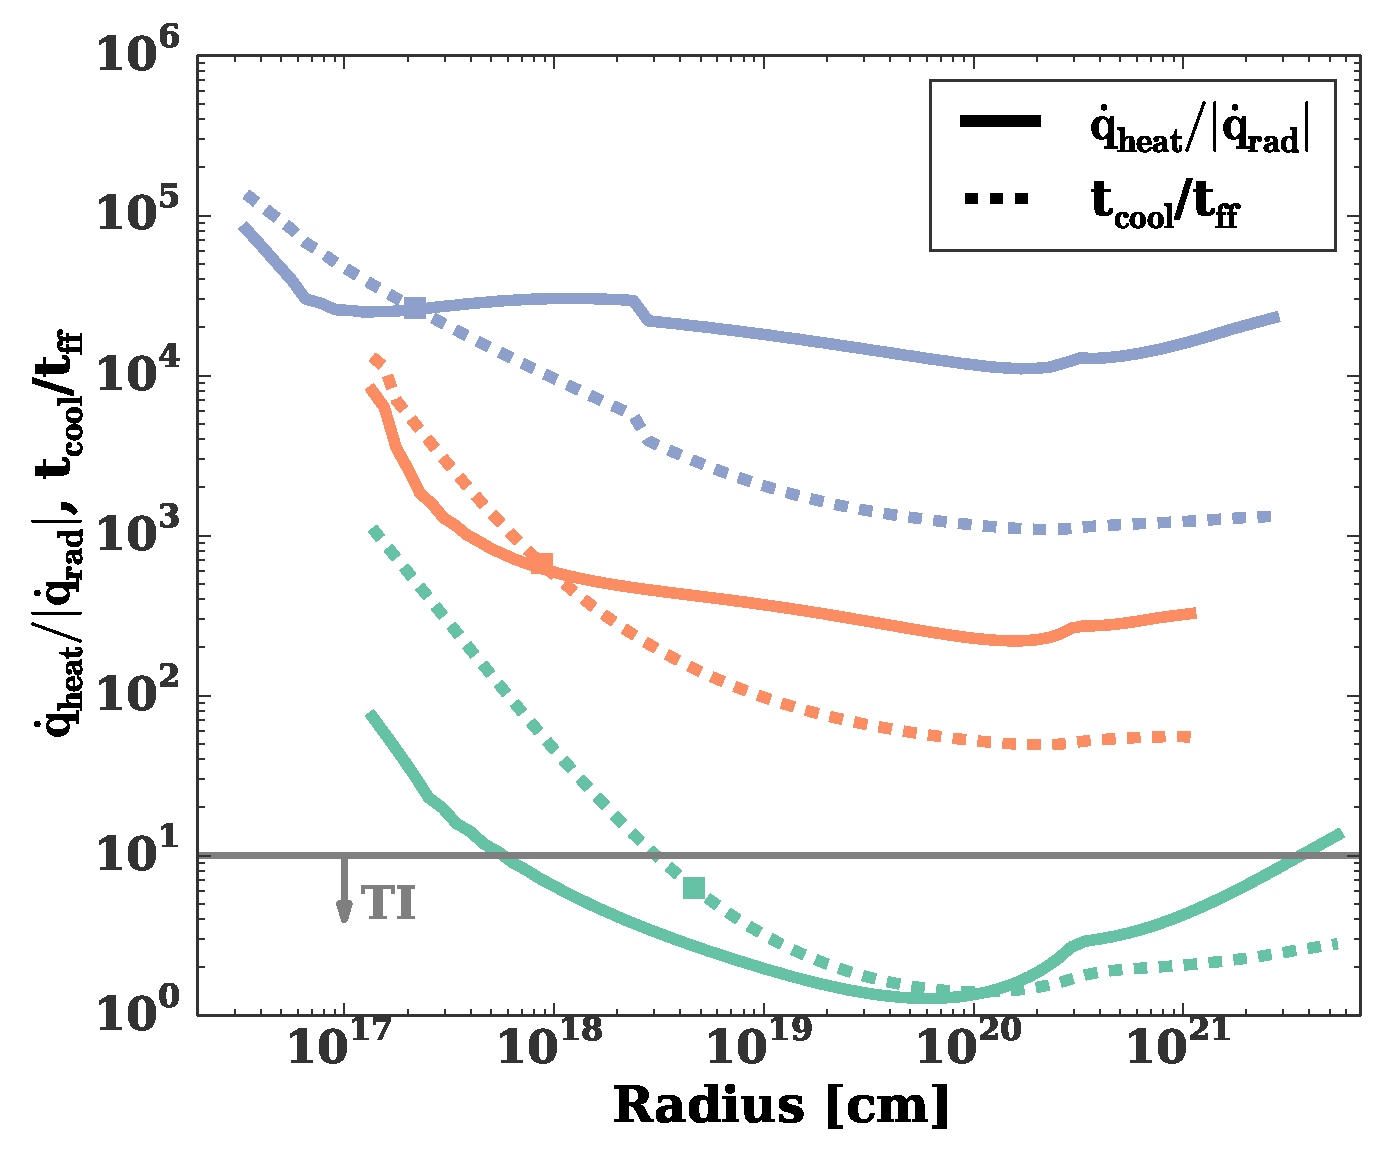
\includegraphics[width=\columnwidth]{cooling.eps}
\caption{\label{fig:cooling} Ratio of heating ($H$) to cooling rate ($C$) for each of our solutions. The cooling rate is calculated using the approximate (solar metallicity) cooling function in Equation~\ref{eq:cooling}. The heating rate is estimated as $q \vw^2/2$. The ratio is computed assuming $eta=1$.}
\end{figure}

For $\vwO$=1000 km/s, it is apparent from Figure~\ref{fig:cooling},
that radiative cooling may be safely neglected. With a few exceptions
this is also true for $\vwO$=500 km/s.  However, for $\vwO$=200 km/s
cooling may be quite important.

For small $\eta$ the effects of cooling will be less pronounced. For
each of our galaxies we give the maximum $\eta$ such that $H/C >$1 in
Table .  Roughly speaking, this is the maximum $\eta$ for which it
would be safe to ignore cooling. $\eta$ depends on the age of the
stellar population, and will realistically vary between $\sim 0.1$ and
$\sim 1$ (see Appendix~\ref{app:eta}).  

For $\vwO$=1000 km/s, it is apparent from Figure~\ref{fig:cooling},
that radiative cooling is negligible. On the other hand, for
$\vwO$=200 km/s radiative cooling would be quite important for many of
our profiles and should be included.

\begin{table}
\begin{tabular}{cccc}
\hline
Galaxy & $\eta_{\rm max}$ $v_{\rm w,0}=$200 km/s & $\eta_{\rm max}$ $v_{\rm w,0}=$500 km/s & $\eta_{\rm max}$ $v_{\rm w,0}=$1000 km/s \\
\hline
NGC1023 & 0.1 & 2.0 & 200.0 \\
NGC1316 &  &  &  \\
NGC4365 &  &  & 100.0 \\
NGC4239 &  &  &  \\
NGC2841 &  &  &  \\
NGC4387 & 0.3 & 90.0 & 5000.0 \\
NGC3115 & 0.2 & 0.7 & 30.0 \\
NGC4621 & 0.3 & 1.0 & 40.0 \\
NGC4564 & 0.1 & 4.0 & 700.0 \\
NGC7768 &  &  &  \\
NGC4464 & 0.3 & 20.0 & 2000.0 \\
NGC4467 & 1.0 & 100.0 & 6000.0 \\
NGC1400 &  &  &  \\
NGC1399 &  &  &  \\
A2052 & 0.02 & 2.0 & 700.0 \\
NGC596 & 0.08 & 9.0 & 1000.0 \\
NGC4889 &  &  &  \\
NGC4472 &  &  &  \\
NGC224 & 0.02 & 4.0 &  \\
NGC5813 & 0.01 &  &  \\
NGC221 & 0.02 & 20.0 & 2000.0 \\
NGC2636 &  &  &  \\
NGC4486b & 0.005 & 0.1 & 50.0 \\
NGC720 &  &  &  \\
NGC1426 & 0.1 & 20.0 & 1000.0 \\
NGC3605 & 0.2 & 80.0 & 5000.0 \\
NGC4434 & 0.07 & 50.0 & 3000.0 \\
NGC4168 &  & 6.0 & 700.0 \\
NGC4636 &  &  &  \\
NGC3608 &  &  &  \\
NGC4551 & 0.1 & 50.0 & 3000.0 \\
NGC4552 &  &  &  \\
NGC4742 &  & 20.0 & 800.0 \\
NGC4478 & 0.03 & 40.0 & 3000.0 \\
NGC4570 & 0.2 & 4.0 & 400.0 \\
NGC4697 & 0.2 & 7.0 & 900.0 \\
NGC1172 &  & 20.0 & 1000.0 \\
NGC4458 & 0.03 & 30.0 & 2000.0 \\
NGC3599 & 0.8 & 200.0 & 9000.0 \\
NGC4874 &  &  &  \\
NGC3377 & 0.02 & 1.0 & 400.0 \\
NGC3379 & 0.02 &  & 200.0 \\
NGC2832 &  &  &  \\
NGC1700 &  &  &  \\
NGC1600 &  &  &  \\
NGC6166 &  &  &  \\
NGC4649 &  &  &  \\
NGC4486 &  & 0.02 &  \\
NGC524 &  &  &  \\
NGC7332 & 0.2 & 20.0 & 2000.0 \\
NGC5845 & 0.06 & 0.3 & 50.0 \\
\end{tabular}
\hline
\end{table}


\subsection{Conduction}
\label{sec:conduction}{

\subsection{Angular Momentum}

\section{Summary}

\appendix
\clearpage
\section{Analytic Expression for the stagnation radius}
\label{app:rs}

Here we derive an analytic expression for the steady-state stagnation radius $r_{\rm s}$.  The steady-state entropy equation (eq.~[\ref{eq:dsdt}]) can be manipulated to read
\begin{align}
T\dsdr=\frac{\Q}{\rho v} \label{eq:ss_entropy}
\end{align}
By definition, the velocity $v$ goes to zero at the stagnation radius.  In order to avoid the entropy derivate from diverging, the numerator of (\ref{eq:ss_entropy}) must also go to zero at $r_{\rm s}$, implying that
\begin{align}
 \frac{\gamma}{\gamma-1} \frac{p|_{\rs}}{\rho|_{\rs}}=\frac{\vw^{2}|_{\rs}}{2} \Rightarrow \frac{\kb T|_{\rs}}{\mu \mp}=\gammafi \frac{\vw^{2}|_{\rs}}{2} .
\label{eq:appTanalytic}
\end{align}
Combining (\ref{eq:ss_entropy}) with the first law of thermodynamics,
\begin{align}
T\dsdr =& \frac{1}{\gamma-1}\ddr{(p/\rho)}-\frac{p}{\rho^2}\ddr{\rho} = \\
& 
\frac{1}{\gamma-1}\left.\ddr{(p/\rho)}\right|_{\rs}+\frac{\densSlope}{\rs}  \frac{p|_{\rs}}{\rho|_{\rs}}=\left.\underbrace{\frac{\Q}{\rho  v}}_{A}\right|_{\rs}, 
% \label{eq:first_law}
\end{align}
where $\densSlope\equiv -\left.d\log(\rho)/d\log(r)\right|_{\rs}$.  The term on the right can be evaluated using L'Hopital's rule, yielding
%\begin{align}
 % &\lim_{r \rightarrow \rs} A=\frac{\lim_{r \rightarrow \rs}
  %  \frac{d}{dr}\left[q (r)\left(\ke -\gammaf
   %     \frac{p}{\rho}+\kew\right)\right]}{\lim_{r \rightarrow \rs}
    %\frac{d}{dr} \left(\rho v\right)}\\
  %&=\frac{ q'|_{\rs} \overbrace{\left.\left(\ke
   %     -\gammaf\frac{p}{\rho}+\kew\right)\right|_{\rs}}^0+ q|_{\rs}
    %\frac{d}{dr} \left[\left(\ke -\gammaf
     %   \frac{p}{\rho}+\kew\right)\right]_{\rs}}{\underbrace{\rho'|_{\rs}
      %v|_{\rs}}_0 +\underbrace{v'|_{\rs}\rho|_{\rs}}_{q|_{\rs}}}\\
\begin{align}
  \lim_{r \rightarrow \rs} A = \frac{d}{dr} \left[\left(\ke -\gammaf \frac{p}{\rho}+\kew\right)\right]_{\rs}
\end{align}
Now using the definition $\vw^2=\vwO^2+ G \Menc/r$, where
$\Menc=\Mbh+\Mstar$, and assuming $\Mstar \sim r^{2-\Gamma}$, we find that
\begin{align}
\lim_{r \rightarrow \rs} A=-\gammaf
\left.\ddr{(p/\rho)}\right|_{\rs}-\frac{G \Menc|_{\rs}}{2 \rs^2}+(2-\Gamma) \frac{G
  \Mstar|_{\rs}}{2 \rs^2}.
\end{align}
Substituting this expression back into equation (\ref{eq:first_law}) and using equation (\ref{eq:appTanalytic}) gives
\begin{align}
&\frac{\gamma+1}{\gamma-1}
\left.\ddr{(p/\rho)}\right|_{\rs}+ \frac{\gamma-1}{\gamma} \frac{\densSlope}{\rs} \vw|_{\rs}^{2} = (2-\Gamma) \frac{G
  \Mstar|_{\rs}}{2 \rs^2} -\frac{G \Menc|_{\rs}}{2 \rs^2}.  \label{eq:rs1}
\end{align}
A second equation results from evaluating the momentum equation (eq.~[\ref{eq:dvdt}]) at the stagnation point
\begin{align}
&\frac{1}{\rho}\dpdr=- \frac{G\Menc}{\rs^2} \Rightarrow
&\ddr{(p/\rho)}+\frac{p}{\rho}
\underbrace{\frac{d\log(\rho)}{dr}}_{-\densSlope/r} = -\frac{G \Menc}{\rs^2} \label{eq:HSE}
\end{align}
Finally, combining equations (\ref{eq:rs1}) and (\ref{eq:HSE}) gives 

\begin{align}
\rs=\frac{G \Mbh}{\densSlope \vw^{2}|_{\rs}}\left(\frac{9-\Gamma}{2}
  \frac{M_{\star}|_{\rs}}{\Mbh} +\frac{7}{2}\right),
\end{align}
where we have assumed $\gamma=5/3$.

In terms of just the additional wind heating parameter, $v_w$,

\begin{align}
\rs=\frac{G \Mbh}{\densSlope v_w^{2}|_{\rs}}\left[\left(\frac{9-\Gamma}{2} -\densSlope\right) \frac{\Mstar|_{\rs}}{\Mbh} +\frac{7}{2}-\densSlope\right].
\label{eq:rs2main}
\end{align}


Defining $\eta \equiv \vwO/\sigma_{\rm soi}$, this relationship can be
reparameterized as follows:
\begin{align}
  \frac{\rs}{\rsoi}=\frac{1}{2 \zeta^2 \densSlope}\left[
    \frac{\Mstar|_{\rs}}{\Mbh}\left(\frac{9-\Gamma}{2}-\densSlope\right)+\left(\frac{7}{2}-\densSlope\right)\right]
\end{align}

%{\bf AG: Note that I have taken sigmainf=2 G Mbh/rinf. Commented out
%equations have sigmainf=G Mbh/rinf}. 
For cusp galaxies ($\Gamma\simeq1$) we have $\Mstar|_{\rs}/\Mbh=x$, $A=4$, and $B=7/2$ for $\gamma = 5/3$, such that 
\begin{align}
\x=\frac{7-2\densSlope}{4\zeta^2 \densSlope+2\densSlope-8}
%\x=\frac{7-2\densSlope}{2\zeta^2 \densSlope+2\densSlope-8}
\end{align}
In the limit of zero wind heating $\eta \rightarrow 0$, no solution
for $r_{\rm s}$ exists unless the gas density profile at the
stagnation radius is steep, 3.5 $<\densSlope<$ 4.

For core galaxies ($\Gamma \simeq 0$) with $\Mstar/\Mbh=x^2$, A=9/2,
and B=7/2, the stagnation radius instead obeys a quadratic equation
\begin{align}
\x=\frac{\zeta^2 \densSlope \pm \sqrt{\zeta^4 \densSlope^2 - \left(\frac{9}{2}-\densSlope\right)
    \left(\frac{7}{2}-\densSlope\right)}}{\left(\frac{9}{2}-\densSlope\right)}
%\x=\frac{\zeta^2 \densSlope \pm \sqrt{\zeta^4 \densSlope^2 - 4 \left(\frac{9}{2}-\densSlope\right)
%\left(\frac{7}{2}-\densSlope\right)}}{2 \left(\frac{9}{2}-\densSlope\right)}
\label{eq:rstag}
\end{align}
In this case no solution exists in the zero heating limit ($\zeta
\rightarrow 0$) unless $3.5<\densSlope<4.5$.

When $\Mstar << \Mbh$ at the stagnation radius, the relationship
between $\rs$ and $\vw$ is greatly simplified.
\begin{align}
\rs=\frac{7}{2}\frac{G \Mbh}{\densSlope \vw^2},
\end{align}
where the pre-factor on the right-hand side corresponds to
$\gamma=5/3$ and $\Gamma=1$ or 0.  



%%% Local Variables:
%%% mode: latex
%%% TeX-master: "ms"
%%% Ennd:


\section{Dependence of q on stellar age}
\label{app:eta}
We now describe the rate of start formation $q$ varies with the age of the stellar population.

If we assume that a stellar population forms impulsively in the distant pass with IMF $\mu(m_*)$(with minimum mass $m_0$ and maximum mass $m_1$), then the surviving mass fraction at any future time $t$ is given by 
\begin{equation}
f(t) =\frac{ \int_{m_0}^{m_{\rm max}(t)} m_* \mu(m_*) dm_* }{ \int_{m_0}^{m_1} m_* \mu(m_*) dm_* },
\end{equation}
where 
\begin{equation}
m_{\rm max}(t) \approx 2.5M_\odot~ \left( \frac{t}{10^9~{\rm yr}} \right)^{-0.4}.
\end{equation}
For a Salpeter IMF $\mu(m_*) \propto m_*^{-2.35}$ with $m_0=0.1M_\odot$ and $m_1=100M_\odot$,
\begin{equation}
f_{\rm Sal}(t) = 1.098 - 0.490 \left(\frac{t}{10^{10}~{\rm yr}} \right)^{0.14}
\end{equation}
%{\bf NCS: we should probably use a Kroupa/Chabrier IMF, but this gets the ball rolling.}
If we approximate post-main sequence evolution as instantaneous and define $\lambda(m_*)$ as the fractional mass lost during all stages of stellar evolution, then the mass loss rate density
\begin{equation}
q(t) = \frac{\rho_*}{\bar{m}_*} \lambda(m_{\rm max}(t)) m_{\rm max}(t) \frac{df}{dt},
\end{equation}
where the mean stellar mass $\bar{m}_* = \int_{m_0}^{m_{\rm max}(t)} m_*\mu(m_*)dm_* \approx 0.3 M_\odot$.  Further approximating $\lambda(m_*)=0.5$, and using the Salpeter IMF once more, gives
\begin{equation}
q(t) = \frac{\rho_*}{\th} \times 0.11 \left(\frac{t}{10^{10}~{\rm yr}} \right)^{-1.26}.
\end{equation}
This is a specific, time-dependent definition of $\eta(t) (=0.11(t/t_{\rm h})^{-1.26})$;

\footnotesize{
  \bibliographystyle{mn2e}
  \bibliography{master}
}
\end{document}
